% Architecture : GLiNER (détection) + têtes de normalisation (ce travail).
% Rendu standalone -> PDF/PNG. Les couleurs Thesis* sont des PLACEHOLDERS : remplace-les
% par celles de ta thèse (mêmes noms) et la figure s'y conforme.
\documentclass[border=6pt]{standalone}
\usepackage{tikz}
\usepackage{amsmath}
\usetikzlibrary{arrows.meta,positioning,fit,backgrounds}

% ---- palette placeholder (à écraser par la vraie) ----
\definecolor{ThesisInk}{RGB}{30,32,40}
\definecolor{ThesisNeutral}{RGB}{120,124,132}
\definecolor{ThesisPrimary}{RGB}{54,96,166}
\definecolor{ThesisPrimaryDark}{RGB}{34,64,120}
\definecolor{ThesisSecondary}{RGB}{72,158,110}
\definecolor{ThesisSecondaryDark}{RGB}{40,110,72}
\definecolor{ThesisTertiary}{RGB}{232,150,98}
\definecolor{ThesisTertiaryDark}{RGB}{190,108,58}
\definecolor{ThesisQuaternary}{RGB}{176,132,204}
\definecolor{ThesisQuaternaryDark}{RGB}{132,86,166}

\begin{document}
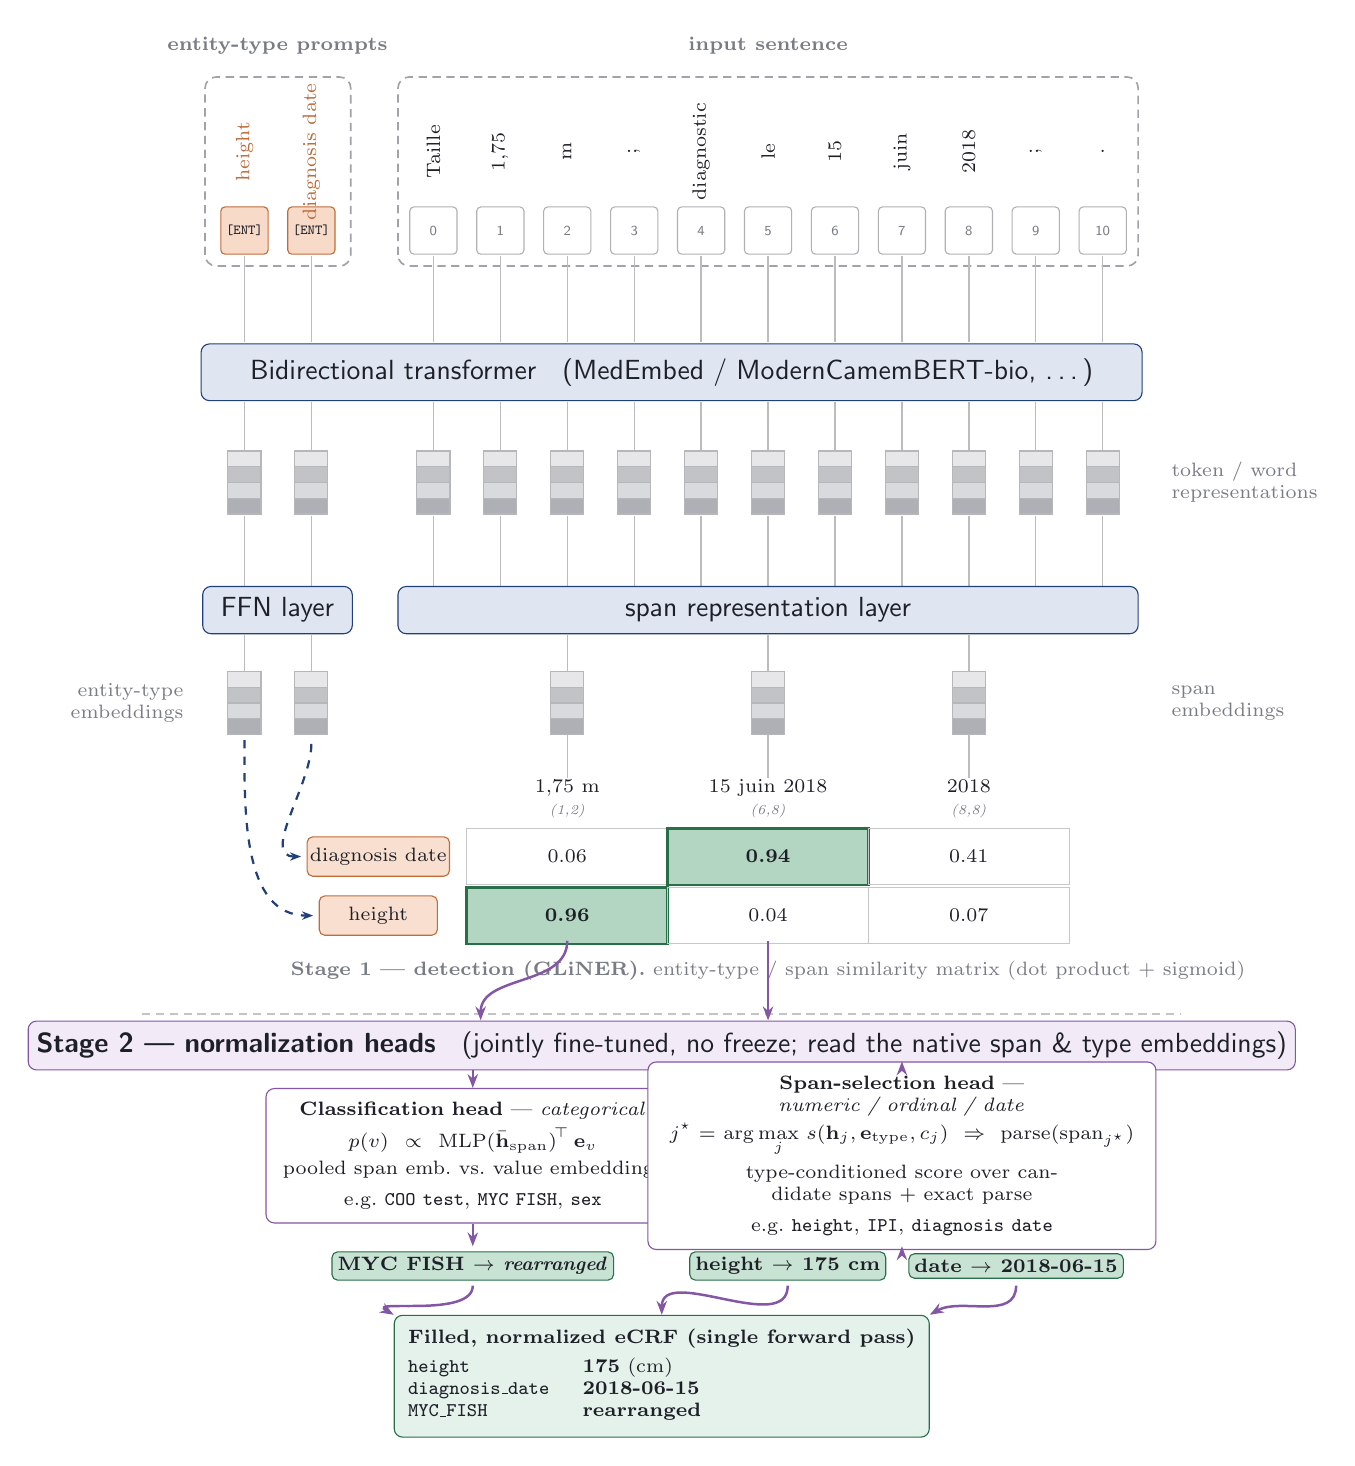
\begin{tikzpicture}[x=1cm,y=1cm, font=\sffamily,
  sq/.style={draw=ThesisInk!35, fill=white, rounded corners=1.5pt,
    minimum size=0.6cm, inner sep=0pt, text=ThesisInk},
  esq/.style={draw=ThesisTertiaryDark, fill=ThesisTertiary!35, rounded corners=1.5pt,
    minimum size=0.6cm, inner sep=0pt, text=ThesisInk,
    font=\fontsize{4.2}{5}\selectfont\ttfamily},
  wlab/.style={rotate=90, font=\scriptsize, text=ThesisInk, inner sep=1pt},
  idx/.style={font=\tiny, text=ThesisNeutral},
  band/.style={draw=ThesisPrimaryDark, fill=ThesisPrimary!16, rounded corners=3pt,
    text=ThesisInk, inner sep=3pt},
  nband/.style={draw=ThesisQuaternaryDark, fill=ThesisQuaternary!16, rounded corners=3pt,
    text=ThesisInk, inner sep=3pt},
  reg/.style={draw=ThesisNeutral!70, densely dashed, rounded corners=4pt, line width=0.6pt},
  conn/.style={ThesisInk!30, line width=0.5pt},
  vcell/.style={draw=ThesisNeutral!55, minimum width=0.42cm, minimum height=0.2cm,
    inner sep=0pt},
  hdr/.style={font=\scriptsize\bfseries, text=ThesisNeutral},
  rlab/.style={font=\scriptsize, text=ThesisNeutral, align=left, anchor=west},
  typechip/.style={draw=ThesisTertiaryDark, fill=ThesisTertiary!30, rounded corners=2pt,
    minimum width=1.5cm, minimum height=0.5cm, inner sep=1pt, text=ThesisInk, font=\scriptsize},
  colhdr/.style={font=\scriptsize, text=ThesisInk, align=center},
  mcell/.style={draw=ThesisInk!25, minimum width=2.55cm, minimum height=0.72cm,
    inner sep=0pt, text=ThesisInk, font=\scriptsize},
  hit/.style={mcell, draw=ThesisSecondaryDark, line width=1pt, fill=ThesisSecondary!42,
    font=\scriptsize\bfseries},
  headbox/.style={draw=ThesisQuaternaryDark, fill=white, rounded corners=3pt,
    inner sep=5pt, text=ThesisInk, align=center, font=\scriptsize},
  valchip/.style={draw=ThesisSecondaryDark, fill=ThesisSecondary!30, rounded corners=2pt,
    inner sep=2pt, text=ThesisInk, font=\scriptsize\bfseries},
  dasharr/.style={dashed, ThesisPrimaryDark, line width=0.8pt,
    -{Stealth[length=4pt]}, shorten >=2pt, shorten <=2pt},
  flow/.style={ThesisQuaternaryDark, line width=0.9pt, -{Stealth[length=5pt]}},
]
\newcommand{\vbar}[2]{%
  \foreach \sh/\yo in {18/0.3,46/0.1,28/-0.1,60/-0.3}{
    \node[vcell, fill=ThesisNeutral!\sh] at (#1,{#2+\yo}) {};}}
\newcommand{\idxlab}[1]{{\tiny\textcolor{ThesisNeutral}{#1}}}
% ============ TOP: region labels + dashed boundaries ============
\node[hdr] at (0.42,2.75) {entity-type prompts};
\node[hdr] at (6.65,2.75) {input sentence};
\draw[reg] (-0.5,-0.05) rectangle (1.35,2.35);
\draw[reg] (1.95,-0.05) rectangle (11.35,2.35);
\foreach \i/\w in {0/height, 1/diagnosis date}{
  \pgfmathsetmacro{\x}{0.85*\i}
  \node[esq] (e\i) at (\x,0.4) {[ENT]};
  \node[wlab, text=ThesisTertiaryDark] at (\x,1.4) {\w};}
\foreach \j/\w in {0/Taille,1/1{,}75,2/m,3/{;},4/diagnostic,5/le,6/15,7/juin,8/2018,9/{;},10/.}{
  \pgfmathsetmacro{\x}{2.4+0.85*\j}
  \node[sq] (s\j) at (\x,0.4) {\idxlab{\j}};
  \node[wlab] at (\x,1.4) {\w};}
\foreach \x in {0,0.85,2.4,3.25,4.1,4.95,5.8,6.65,7.5,8.35,9.2,10.05,10.9}{
  \draw[conn] (\x,0.08) -- (\x,-1.02);}
% ============ TRANSFORMER band ============
\node[band, minimum width=11.95cm, minimum height=0.72cm] (tf) at (5.425,-1.4)
  {Bidirectional transformer \; (MedEmbed / ModernCamemBERT-bio, \dots)};
\foreach \x in {0,0.85,2.4,3.25,4.1,4.95,5.8,6.65,7.5,8.35,9.2,10.05,10.9}{
  \draw[conn] (\x,-1.78) -- (\x,-2.42);}
\foreach \x in {0,0.85,2.4,3.25,4.1,4.95,5.8,6.65,7.5,8.35,9.2,10.05,10.9}{ \vbar{\x}{-2.8} }
\node[rlab] at (11.65,-2.8) {token / word\\ representations};
\foreach \x in {0,0.85}{ \draw[conn] (\x,-3.22) -- (\x,-4.12); }
\foreach \x in {2.4,3.25,4.1,4.95,5.8,6.65,7.5,8.35,9.2,10.05,10.9}{
  \draw[conn] (\x,-3.22) -- (\x,-4.12); }
\node[band, minimum width=1.9cm, minimum height=0.6cm] (ffn) at (0.42,-4.42) {FFN layer};
\node[band, minimum width=9.4cm, minimum height=0.6cm] (spn) at (6.65,-4.42)
  {span representation layer};
\foreach \x in {0,0.85}{ \draw[conn] (\x,-4.72) -- (\x,-5.22); \vbar{\x}{-5.6} }
\node[rlab, anchor=east, text width=1.7cm, align=right] at (-0.65,-5.6)
  {entity-type\\ embeddings};
\foreach \x in {4.1,6.65,9.2}{ \draw[conn] (\x,-4.72) -- (\x,-5.22); \vbar{\x}{-5.6} }
\node[rlab] at (11.65,-5.6) {span\\ embeddings};
\foreach \x in {4.1,6.65,9.2}{ \draw[conn] (\x,-6.0) -- (\x,-6.55); }
% ============ similarity matrix (STAGE 1: detection, GLiNER) ============
\node[colhdr] at (4.1,-6.82) {1{,}75 m\\ {\tiny\itshape\textcolor{ThesisNeutral}{(1,2)}}};
\node[colhdr] at (6.65,-6.82) {15 juin 2018\\ {\tiny\itshape\textcolor{ThesisNeutral}{(6,8)}}};
\node[colhdr] at (9.2,-6.82) {2018\\ {\tiny\itshape\textcolor{ThesisNeutral}{(8,8)}}};
\node[typechip] (ra) at (1.7,-7.55) {diagnosis date};
\node[typechip] (rb) at (1.7,-8.30) {height};
\node[mcell] at (4.1,-7.55) {0.06};
\node[hit]   at (6.65,-7.55) {0.94};
\node[mcell] at (9.2,-7.55) {0.41};
\node[hit]   at (4.1,-8.30) {0.96};
\node[mcell] at (6.65,-8.30) {0.04};
\node[mcell] at (9.2,-8.30) {0.07};
\draw[dasharr] (0.85,-6.05) to[out=-90,in=180] (ra.west);
\draw[dasharr] (0,-6.0) to[out=-90,in=180] (rb.west);
\node[font=\scriptsize, text=ThesisNeutral] at (6.65,-9.0)
  {\textbf{Stage 1 — detection (GLiNER).} entity-type / span similarity matrix (dot product $+$ sigmoid)};

% ================================================================
% ============ STAGE 2 : NORMALIZATION HEADS (this work) =========
% ================================================================
\draw[ThesisNeutral!45, densely dashed, line width=0.6pt] (-1.3,-9.55) -- (11.9,-9.55);
\node[nband, minimum width=13.0cm, minimum height=0.62cm] (nb) at (5.3,-9.95)
  {\textbf{Stage 2 — normalization heads} \; (jointly fine-tuned, no freeze; read the native span \& type embeddings)};
% flux depuis les entités reconnues + embeddings vers les têtes
\draw[flow] (6.65,-8.62) -- (6.65,-9.63);
\draw[flow] (4.1,-8.62) to[out=-90,in=90] (3.0,-9.63);

% --- head A : classification (categorical fields) ---
\node[headbox, text width=4.9cm] (hA) at (2.9,-11.35)
  {\textbf{Classification head} — \emph{categorical}\\[2pt]
   $\displaystyle p(v)\propto \mathrm{MLP}(\bar{\mathbf{h}}_{\text{span}})^{\!\top}\,\mathbf{e}_v$\\[2pt]
   {\scriptsize pooled span emb.\ vs.\ value embeddings}\\[3pt]
   {\scriptsize e.g.\ \texttt{COO test}, \texttt{MYC FISH}, \texttt{sex}}};
\node[valchip] at (2.9,-12.75) {MYC FISH $\rightarrow$ \textit{rearranged}};

% --- head B : span selection (numeric / ordinal / date) ---
\node[headbox, text width=6.1cm] (hB) at (8.35,-11.35)
  {\textbf{Span-selection head} — \emph{numeric / ordinal / date}\\[2pt]
   $\displaystyle j^\star=\arg\max_j\, s(\mathbf{h}_j,\mathbf{e}_{\text{type}},c_j)\;\Rightarrow\;\mathrm{parse}(\text{span}_{j^\star})$\\[2pt]
   {\scriptsize type-conditioned score over candidate spans $+$ exact parse}\\[3pt]
   {\scriptsize e.g.\ \texttt{height}, \texttt{IPI}, \texttt{diagnosis date}}};
\node[valchip] at (6.9,-12.75) {height $\rightarrow$ \textbf{175} cm};
\node[valchip] at (9.8,-12.75) {date $\rightarrow$ \textbf{2018-06-15}};

\draw[flow] (nb.south-|2.9,0) ++(0,0) -- (hA.north);
\draw[flow] (nb.south-|8.35,0) ++(0,0) -- (hB.north);
\draw[flow] (hA.south) -- (2.9,-12.5);
\draw[flow] (hB.south) -- (8.35,-12.5);

% --- output : filled normalized eCRF ---
\node[draw=ThesisSecondaryDark, fill=ThesisSecondary!14, rounded corners=3pt,
      inner sep=5pt, align=left, font=\scriptsize, text=ThesisInk] (ecrf) at (5.3,-14.15)
  {\textbf{Filled, normalized eCRF (single forward pass)}\\[2pt]
   \begin{tabular}{@{}ll@{}}
     \texttt{height} & \textbf{175} (cm)\\
     \texttt{diagnosis\_date} & \textbf{2018-06-15}\\
     \texttt{MYC\_FISH} & \textbf{rearranged}\\
   \end{tabular}};
\draw[flow] (2.9,-13.0) to[out=-90,in=150] (ecrf.north west);
\draw[flow] (6.9,-13.0) to[out=-90,in=90] (ecrf.north);
\draw[flow] (9.8,-13.0) to[out=-90,in=30] (ecrf.north east);
\end{tikzpicture}
\end{document}
